% !TEX encoding = UTF-8
% !TEX TS-program = pdflatex
% !TEX root = ../tesi.tex

%**************************************************************
\chapter{Integrazione di Amazon Rekognition}
\label{cap:rekognition}
%**************************************************************

In questo capitolo viene approfondito lo sviluppo e l'integrazione del sistema di image recognition\\

%**************************************************************

\section{Presentazione del problema}
MariBa è una piattaforma per il salvataggio dei risultati delle partite giocate dai dipendenti di \azienda durante le 
pause pranzo e caffè. \\
L'inizializzazione di una partita prevede l'inserimento dei nomi di tutti i giocatori, specificando anche la posizione (attacco o difesa) e le squadre nel caso del calcetto balilla. Questo procedimento di inserimento dei dati iniziali
risultava laborioso ed è stata quindi espressa la necessità di velocizzare tale procedura. \\
L'idea è quella di scattare una foto ai giocatori partecipanti in modo tale che l'applicazione li riconosca in modo automatico.

\section{Progettazione}
Di seguito viene descritta la progettazione ed il funzionamento della funzionalità di riconoscimento facciale implementata.
	\subsection{Architettura}
	Di seguito vengono descritte in modo approfondito le componenti sviluppate per il servizio di image recognition, i servizi utilizzati e come essi lavorino insieme per il raggiungimento dell'obiettivo. \\
	
	\subsubsection{Amazon Rekognition}
	
	\emph{Amazon Rekognition} è un software \emph{cloud-based} che mette a disposizione capacità di visione artificiale pre-addestrate e personalizzabili per estrarre informazioni dettagliate da immagini e video. Nel caso del progetto è stato utilizzato per indicizzare le facce e permetterne quindi il riconoscimento. In particolare, tutte le facce sono state salvate all'interno di una raccolta (\emph{collection}) e a ciascuna di esse è stato assegnato un ID univoco (\emph{faceId}). Per effettuare un riconoscimento si procede ad una ricerca di eventuali corrispondenze all'interno di tale \emph{collection} . \\
	Di seguito sono elencate le funzioni utilizzate:
	\begin{itemize}
		\item \texttt{DetectFaces}: individua le cento facce di dimensione maggiore presenti nell'immagine. Per ogni viso individuato ne restituisce i dettagli, in particolare la \emph{bounding box};
		\item \texttt{IndexFaces}: Individua i visi all'interno di un'immagine e li aggiunge ad una \emph{collection} specificata. Per questioni di sicurezza \emph{Rekognition} non salva direttamente l'immagine contenente la faccia ma ne salva solamente le caratteristiche che ne permettano il riconoscimento.
		\item \texttt{SearchFacesByImage}: data un'immagine, vengono identificate le facce presenti e successivamente ne vengono cercate delle corrispondenze all'interno di una \emph{collection} specificata.
		
	\end{itemize} 
	
	\subsubsection{S3}
	descrizione del bucket con la lifecycle rule
	
	\emph{Amazon Simple Storage Service} (S3) è un servizio di archiviazione oggetti. Al suo interno i dati sono organizzati in \emph{bucket}. All'interno di ogni \emph{bucket} è possibile definire dei prefissi per poter organizzare al meglio gli oggetti caricati. \\ Per evitare un passaggio diretto delle immagini tra front-end e back-end si è utilizzato questo servizio. S3 infatti fornisce la possibilità di generare un URL per effettuare operazione in una specifica posizione all'interno del \emph{bucket}.
	
	\subsubsection{AWS Lamda}
	descrizione delle lambda e di come vengono utilizzate
	
	
	
	\subsection{Funzionamento generale}
	% grafico funzionamento
	\begin{itemize}
		\item front-end richiede url per caricamento
		\item caricamento su s3
		\item chiamata callRekognition
		\item scarica l'immagine e chiama elaborateImage
		\item chiama rekognition.detectFaces per l'individuazione dei visi
		\item per ciascuno dei visi chiama rekognition.searchFaceByImage per il riconoscimento 
		\item per i visi riconosciuti restituisce il faceid della faccia il cui match ha maggiore confidenza
		\item per i visi non riconosciuti restituisce il crop della foto per permettere un'eventuale indicizzazione in caso di richiesta
		\item ritorna i dati a callRekognition
		\item callRekognition torna al frontend i dati 
		\item il front-end li visualizza
		
		\item Se viene richiesto di registrare un nuovo utente:\\
		il crop viene indicizzato nella collection di rekognition\\
		viene restituito il faceId del viso indicizzato \\
		il nuovo utente viene registrato con il faceId ricevuto in modo che la volta successiva possa essere riconosciuto direttamente
		
		\item Se viene richiesto di associare un nickname già esistente ad un viso:
		il crop della foto viene indicizzato\\
		viene restituito il faceId\\
		viene aggiornato il record dell'utente selezionato aggiungendo o sostituendo il faceId
	\end{itemize}
	
		
		
	
	
	\subsection{Design dell'interfaccia}
	Per il design dell'interfaccia, prima della sua effettiva codifica, sono stati realizzati dei \emph{wireframes} utilizzando \textbf{Balsamiq} che definissero il flusso di funzionamento a livello di front-end. \\ 

	\noindent Successivamente, la realizzazione dell'interfaccia è avvenuta utilizzando \textbf{Angular 12.x} in combinazione con la libreria 
	\textbf{Nebular}, specifica per lo sviluppo di interfacce utente. \\
	Il procedimento di inserimento dei giocatori è leggermente differente a seconda del gioco utilizzato.
	
		\subsubsection{Inserimento di una nuova partita di calcetto}
		Nella pagina per l'inizializzazione di una nuova partita di calcetto è stato aggiunto un pulsante per attivare la webcam e scattare la foto  contenente i volti dei giocatori (\autoref{fig:calcetto-1}). Lo scatto viene quindi inviato a \emph{Amazon Rekognition} per il riconoscimento. 
		
		\begin{figure}[H]
			\centering
			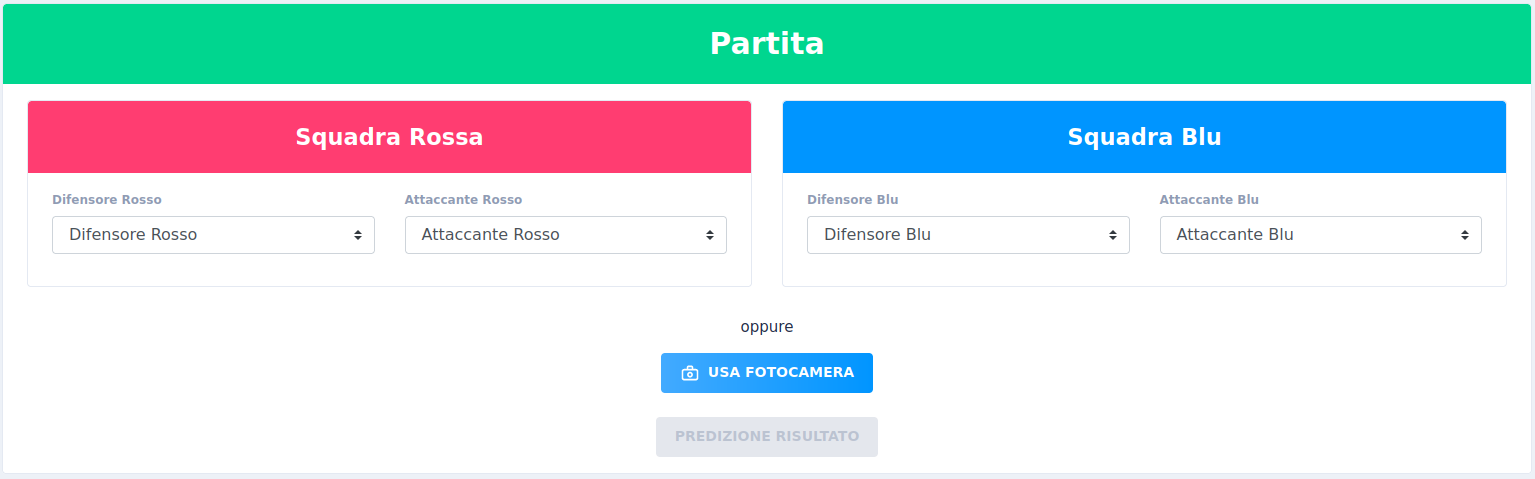
\includegraphics[width=\textwidth]{immagini/calcetto-1.png} \\
			\caption{\label{fig:calcetto-1} Schermata iniziale di calcetto}
		\end{figure}
	
		\noindent Una volta ricevuto il risultato dell'elaborazione, i giocatori vengono visualizzati in card selezionabili per la formazione delle squadre (\autoref{fig:calcetto-2}). I giocatori possono appartenere a tre categorie differenti:
		\begin{itemize}
			\item \textbf{Giocatore riconosciuto}: viene mostrato il nickname corrispondente al volto riconosciuto;
			\item \textbf{Giocatore non riconosciuto ma registrato}: quando selezionato richiede l'associazione del nickname al viso scegliendo tra i nickname già presenti nel database; 
			\item\textbf{Giocatore non riconosciuto e non registrato}: quando selezionato richiede la registrazione di un nuovo giocatore; 
		\end{itemize}
	
		\noindent Nel caso in cui uno o più giocatori non fossero presenti all'interno della fotografia scattata, è possibile inserirli manualmente. Una volta inserito il nickname desiderato, viene mostrata la card corrispondente. \\
		Il numero di giocatori selezionabili per ciascuna squadra è esattamente due. 
		
		\begin{figure}[H]
			\centering
			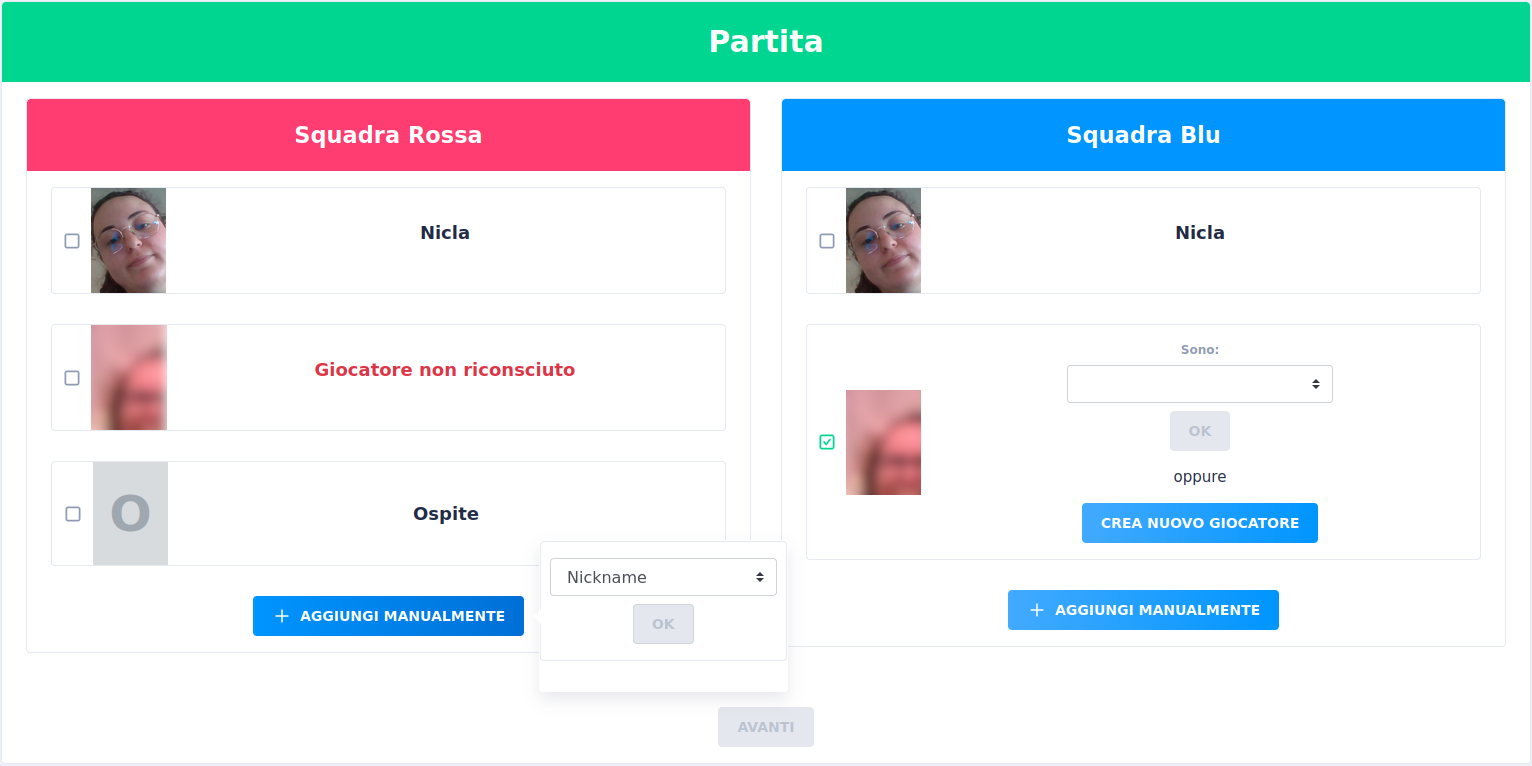
\includegraphics[width=\textwidth]{immagini/calcetto-2.png} \\
			\caption{\label{fig:calcetto-2} Selezione dei giocatori}
		\end{figure}
		
		\noindent Dopo la selezione dei giocatori sarà possibile scambiare i due nickname all'interno di ciascuna squadra per associare loro il ruolo desiderato e formare le squadre definitive (\autoref{fig:calcetto-3}) .
			
		\begin{figure}[H]
			\centering
			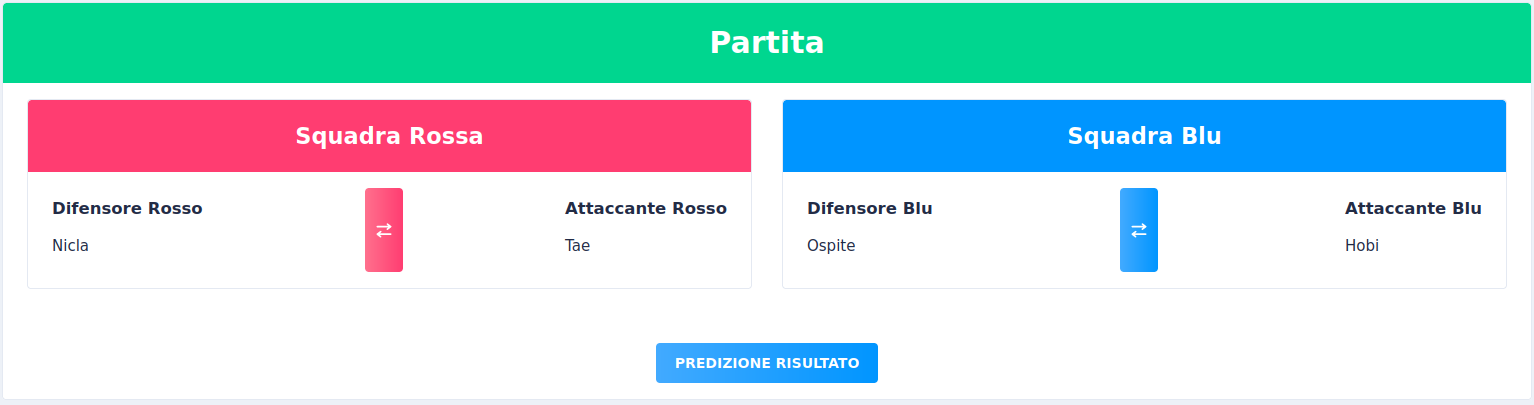
\includegraphics[width=\textwidth]{immagini/calcetto-3.png} \\
			\caption{\label{fig:calcetto-3} Formazione squadre di calcetto}
		\end{figure}
		
		
		\subsubsection{Inserimento di una nuova partita di Mario Kart e Duck Game}
		Il procedimento da seguire per l'inserimento di una partita di Mario Kart o di Duck Game tramite l'utilizzo del riconoscimento facciale dei giocatori è pressoché il medesimo. \\
		La sola differenza tra i due giochi è individuabile nel numero di giocatori selezionabili: 
		\begin{itemize}
			\item per Mario Kart devono essere inseriti esattamente quattro giocatori (\autoref{fig:kart-1});
			\item per Duck Game si possono inserire da un minimo di due ad un massimo di otto giocatori (\autoref{fig:duck-1}).
		\end{itemize}
	
		Ad entrambe le schermate, come per calcetto, è stato quindi aggiunto un pulsante per attivare la webcam e scattare la fotografia da inviare ad \emph{Amazon Rekognition}.
		
		\begin{figure}[H]
			\centering
			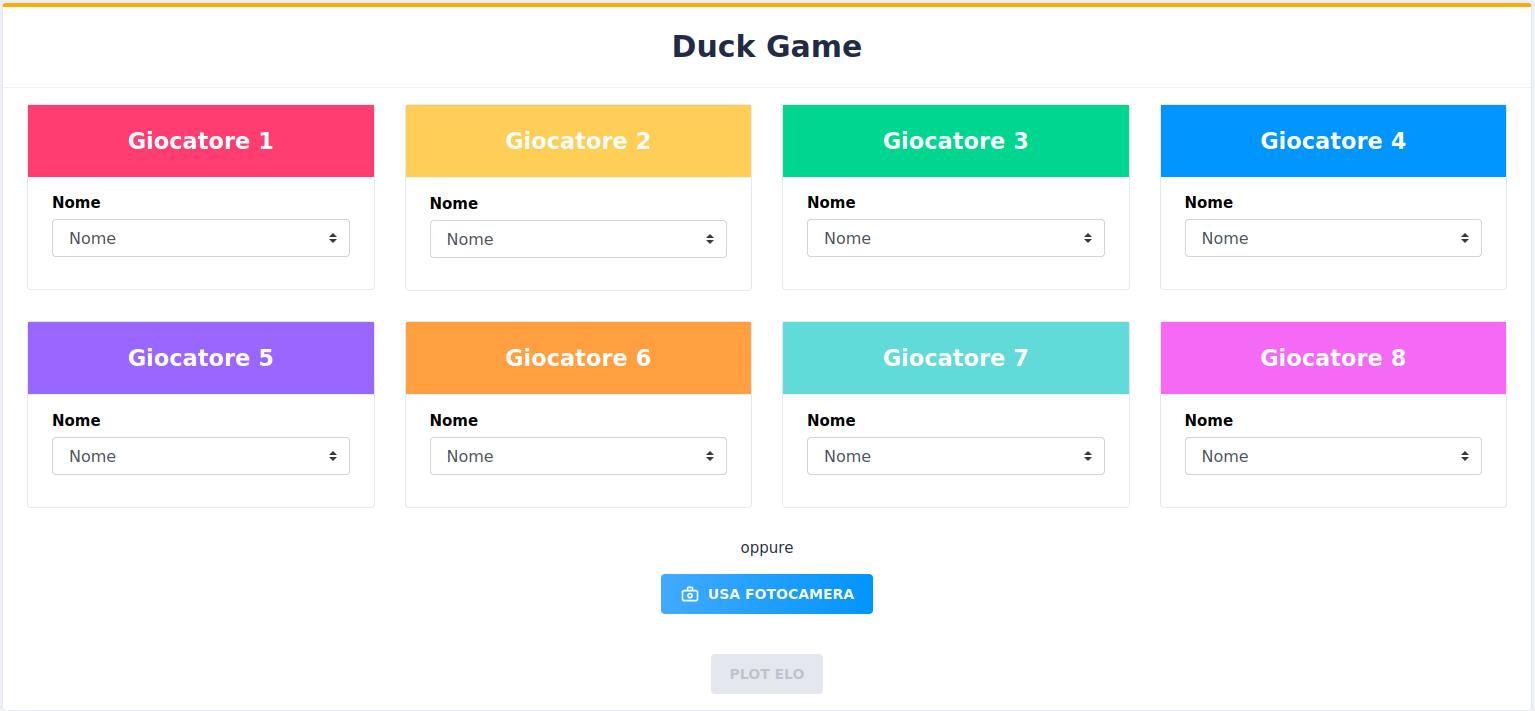
\includegraphics[width=\textwidth]{immagini/duck-1.png} \\
			\caption{\label{fig:duck-1} Schermata iniziale di Duck Game}
		\end{figure}
	
		\begin{figure}[H]
			\centering
			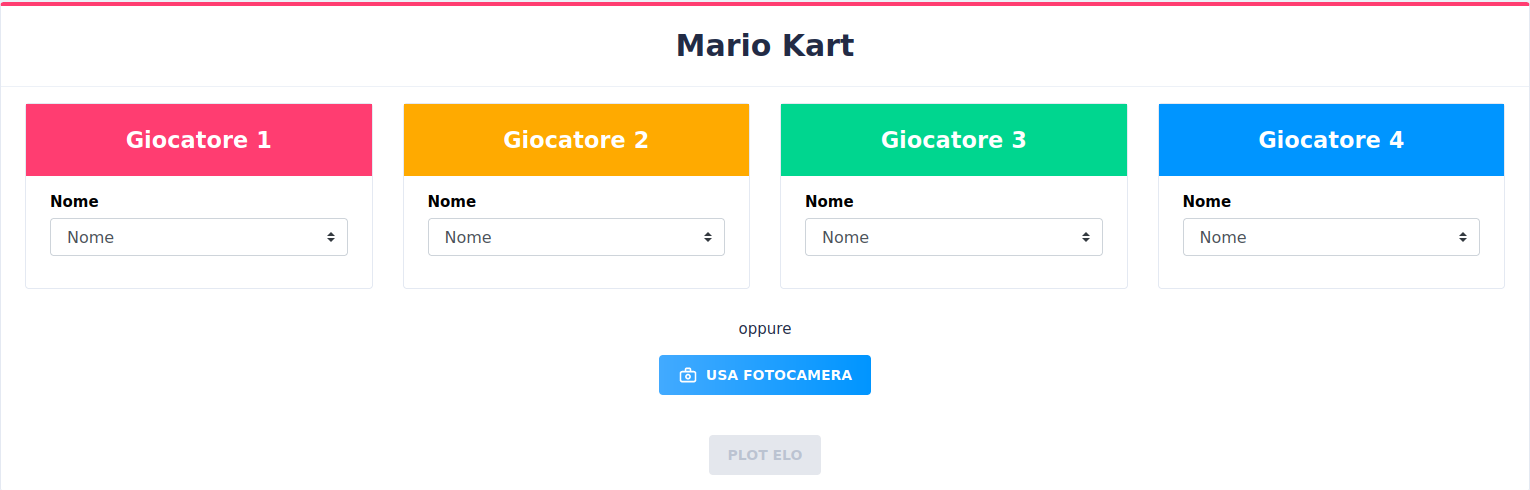
\includegraphics[width=\textwidth]{immagini/kart-1.png} \\
			\caption{\label{fig:kart-1} Schermata iniziale di Mario Kart}
		\end{figure}
		
		\noindent Una volta ricevuto il risultato dell'elaborazione, i giocatori vengono visualizzati in card selezionabili per la formazione delle squadre (\autoref{fig:kart-2}). I giocatori possono appartenere a tre categorie differenti:
		\begin{itemize}
			\item \textbf{Giocatore riconosciuto}: viene mostrato il nickname corrispondente al volto riconosciuto;
			\item \textbf{Giocatore non riconosciuto ma registrato}: il giocatore è già registrato ma non ha ancora volto associato. Quando selezionato richiede l'associazione del nickname al viso scegliendo tra i nickname già presenti nel database; 
			\item\textbf{Giocatore non riconosciuto e non registrato}: quando selezionato richiede la registrazione di un nuovo giocatore; 
		\end{itemize} 
	
		\noindent Nel caso in cui uno o più giocatori non fossero presenti all'interno della fotografia scattata, è possibile inserirli manualmente. Una volta inserito il nickname desiderato, viene mostrata la card corrispondente.
		
		\begin{figure}[H]
			\centering
			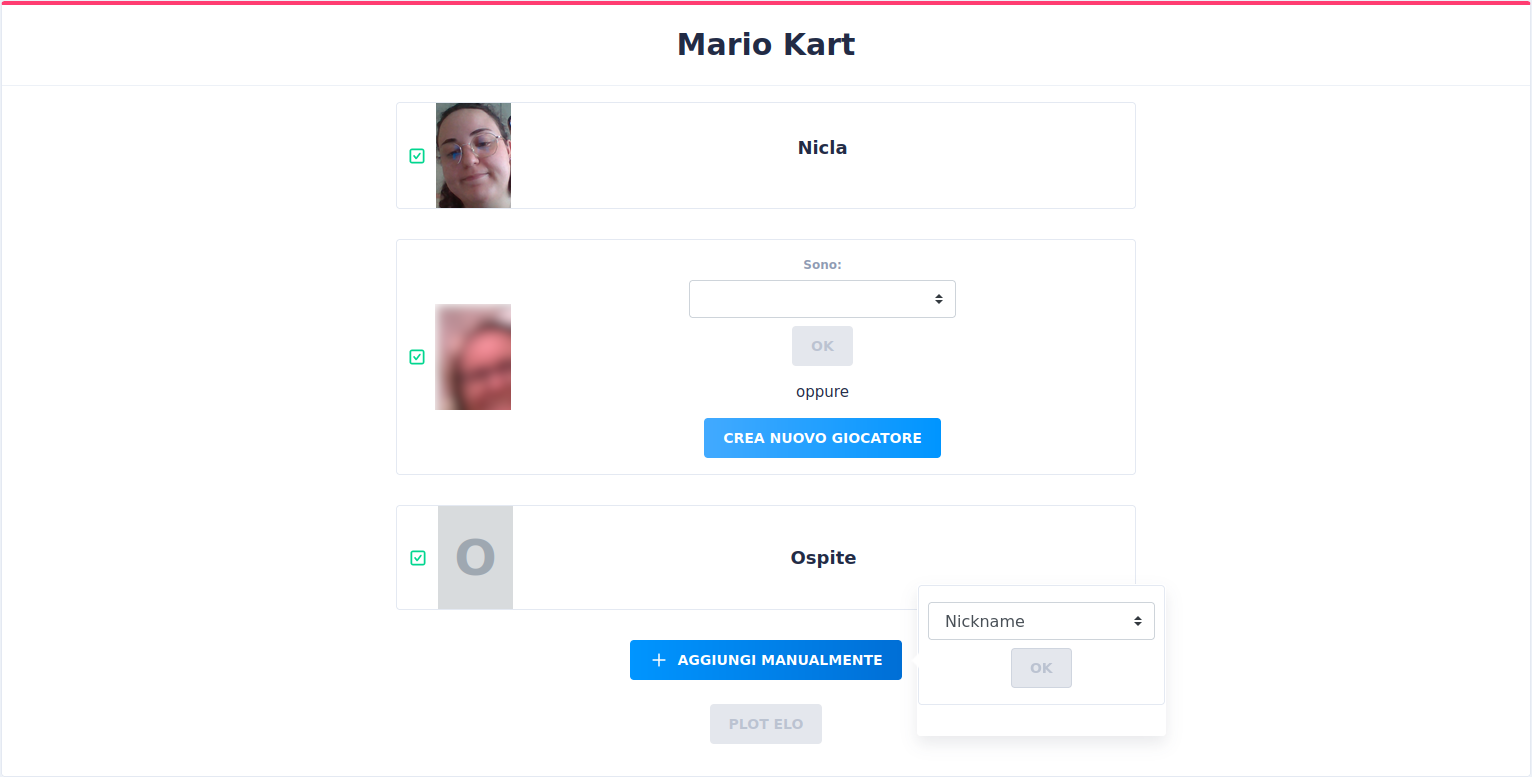
\includegraphics[width=\textwidth]{immagini/kart-2.png} \\
			\caption{\label{fig:kart-2} Selezione dei giocatori di Mario Kart}
		\end{figure}
	
		
